% ==============================================
% SEÇÃO: INTRODUÇÃO
% ==============================================
\section{Introdução}
\label{sec:introducao}

\vspace{1cm}

Este trabalho tem como objetivo estudar uma ligação de rádio completa,
composta por transmissor, canal e recetor, abordando-a em três níveis:
simulação de sistema, simulação de circuito e medição experimental.

Na primeira parte simula-se uma ligação AM no \textit{GNU Radio Companion},
com uma portadora entre 50 e 100~kHz, seguindo o diagrama de blocos da
Figura~\ref{fig:diagrama_am}. No transmissor, a mensagem é escalada pelo
índice de modulação $m$, somada a uma componente contínua, multiplicada pela
portadora e amplificada pelo PA. O canal acrescenta ruído de nível ajustável.
No recetor, o sinal é desconvertido por um misturador em quadratura (I/Q) e
filtrado, e a mensagem é recuperada a partir das componentes I e Q. O sistema
é testado com uma sinusoide de 1~kHz e com um ficheiro de áudio, e avalia-se o
efeito do ruído na relação sinal-ruído (SNR).

\begin{figure}[htbp]
  \centering
  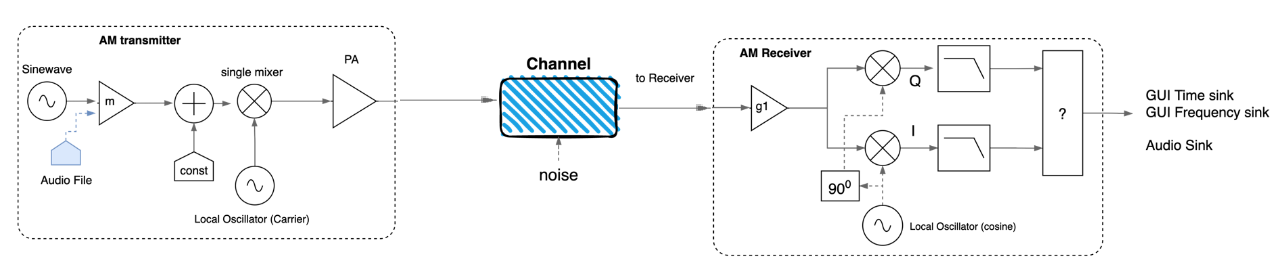
\includegraphics[width=\textwidth]{IMAGENS/lab1_intro.png}
  \caption{Diagrama de blocos simplificado da ligação AM simulada}
  \label{fig:diagrama_am}
\end{figure}

Na segunda parte implementa-se a mesma ligação em LTspice, ao nível de
circuito. A mistura é feita com interruptores comandados por um oscilador
local de onda quadrada e a amplificação com um andar de fonte comum.
Os resultados são comparados com os obtidos no GNU Radio.

Na terceira parte projeta-se um filtro passa-banda LC de 2.\textordfeminine{}
ordem para a banda FM, que é simulado com componentes ideais e reais e medido
com um nanoVNA. O filtro é depois integrado num recetor FM \textit{low-IF},
composto por um LNA, um misturador AD831 e um sintetizador PLL ADF4351, com
desmodulação final em GNU Radio através da plataforma ADALM2000.

